\ifdefined \buildingFullOPALManual \else


%\ifx \@buildingFullOPALManual \@empty
%\else

%\documentclass[12pt,a4paper]{report}
\documentclass[a4paper]{book}

%% does not work in Latex2Html mode
%\usepackage{hyperref}

\usepackage[T1]{fontenc}
\usepackage{url}
\usepackage{html}
\usepackage{epic}
\usepackage{eepic}
\usepackage{makeidx}
\usepackage{array}
\usepackage{times}
\usepackage{amsmath}
\usepackage{amsxtra}
\usepackage{bm}
\usepackage[thin,thinp,thinc]{esdiff}
\usepackage{graphicx}
\usepackage{dingbat}
\usepackage{color}
\usepackage{subfig}
\usepackage{boxedminipage}
\usepackage{alltt}
\usepackage{nicefrac}
\usepackage{calc}
%\usepackage{pdfdraftcopy}             % Draft
\usepackage{tikz}
\usetikzlibrary{
  er,3d,calc,fadings,trees,positioning,arrows,chains,decorations.pathreplacing,
  decorations.pathmorphing,shapes,shapes.symbols,shapes.arrows,matrix,through,decorations.text
}

\tikzset{
  >=stealth',
  punktchain/.style={rectangle,rounded corners, draw=black, very thick,text width=10em,
                     minimum height=3em, text centered, on chain},
  line/.style={draw, thick, <-},
  element/.style={tape,top color=white,bottom color=blue!50!black!60!,minimum width=8em,
                  draw=blue!40!black!90, very thick,text width=10em, minimum height=3.5em,
                  text centered, on chain},
  every join/.style={->, thick,shorten >=1pt},
  tuborg/.style={decorate},
  tubnode/.style={midway, right=2pt}
}

\tikzstyle{material}=[draw, fill=blue!20, text width=16.0em, text centered, minimum height=1.5em]
\tikzstyle{diagramstep} = [material, text width=20em, minimum width=10em, minimum height=3em, rounded corners]
\tikzstyle{line} = [draw, thick, color=black!50, -latex']

\usepackage{booktabs}
\usepackage{xspace}
\usepackage{xstring}

\usepackage{fancyvrb}
\usepackage{rotating}
\usepackage{float}

\usepackage{tabularx}
\usepackage{longtable}
\setcounter{LTchunksize}{3}

\usepackage[section]{placeins}
\usepackage{MnSymbol}
\usepackage{microtype}
\usepackage{setspace}
\usepackage{dcolumn}

\usepackage[vmargin={3.0cm,3.0cm},
            hmargin={2.0cm,3.0cm}]{geometry}

\usepackage{upgreek}
\usepackage[binary-units=true]{siunitx}
\sisetup{exponent-product = \cdot,math-ohm=\Upomega,text-ohm=\ensuremath{\Upomega}}
\DeclareSIUnit{\clight}{c}
\DeclareSIUnit\gauss{Ga}

\usepackage{engord}
\usepackage{wasysym}
\DeclareSIUnit[number-unit-product = \,]{\permill}{\permil}

\usepackage{hyperref}
\hypersetup{
    pdftitle          = The OPAL Framework,
    pdfauthor         = {Andreas Adelmann, Achim Gsell, Valeria Rizzoglio, Christof Metzger-Kraus,
                         Yves Ineichen, Xiaoying Pang, Steve Russell, Chuan Wang, Jianjun Yang,
                         Suzanne Sheehy, Chris Rogers, Daniel Winklehner},
    pdfsubject        = User's Reference Manual,
    pdffitwindow      = true,               % page fit to window when opened
    pdfnewwindow      = true,               % links in new window
    colorlinks        = true,               % false: boxed links; true: colored links
    linkcolor         = black!80!green,     % color of internal links
    citecolor         = black!20!red,       % color of links to bibliography
    urlcolor          = blue,               % color of external links
    breaklinks        = true,
    bookmarksnumbered = true,
    plainpages        = false
}

\usepackage{ifthen}

\newif \iflinuxwindows
\linuxwindowstrue   % set this to true when building the manual on Linux or Windows
\iflinuxwindows
\usepackage{epstopdf}
\fi

\usepackage[backend=biber,
            style=phys,
            biblabel=brackets,
            maxnames=3,
            doi=true,
            isbn=true,
            url=true]{biblatex}
%---- macros ----

\renewcommand{\topfraction}{1.0}
\renewcommand{\bottomfraction}{1.0}
\renewcommand{\textfraction}{0.0}
\renewcommand{\arraystretch}{2.0}
\newenvironment{tex2html_nowrap}{}{}


\newcommand{\Newline}{\hfil \\}


\newsavebox{\ExampleBox}
\newenvironment{example}
 {\VerbatimEnvironment
  \begin{flushleft}
  \begin{lrbox}{\ExampleBox}
    \begin{minipage}{\linewidth}
  \begin{Verbatim}[frame=lines,xleftmargin=0cm,fontsize=\footnotesize,samepage=true]}
 {\end{Verbatim}
  \end{minipage}
  \end{lrbox}
  \mbox{\usebox{\ExampleBox}}
  \end{flushleft}
 }

\newenvironment{longexample}
{\Verbatim[frame=lines,xleftmargin=0mm,fontsize=\footnotesize]}
{\endVerbatim}

%\examplefromfile{filename} reads in a text file and displays it in the document.
\newcommand{\examplefromfile}[1]{
\VerbatimInput[frame=lines,xleftmargin=0mm,fontsize=\footnotesize,label=\texttt{#1}]{#1}}

%for upright d of differentials
\makeatletter
\newcount\my@repeat@count

\newcommand{\myrepeat}[2]{%
  \begingroup
  \my@repeat@count=\z@
  \@whilenum\my@repeat@count<#1\do{#2\advance\my@repeat@count\@ne}%
  \endgroup
}

\newcommand{\differential}[1]{\ifstrempty{#1}{\ES@dop\ES@difint}{\ES@dop^{#1}\ES@difint}}
\newcommand{\pdifferential}[1]{\ifstrempty{#1}{{\partial\,}}{{\partial^{#1}\,}}}

\makeatother

\newcommand{\der}[3][]{\frac{\differential{#1}#2}{\differential{}\ifstrempty{#1}{#3}{#3^#1}}}
\newcommand{\parder}[3][]{\frac{\pdifferential{#1}#2}{\pdifferential{}\ifstrempty{#1}{#3}{#3^#1}}}
\newcommand{\niceder}[3][]{\nicefrac{\differential{#1}#2}{\differential{}\ifstrempty{#1}{#3}{#3^#1}}}
\newcommand{\uglyder}[3][]{{\differential{#1}#2}/{\differential{}\ifstrempty{#1}{#3}{#3^#1}}}
\newcommand{\uglyparder}[3][]{{\pdifferential{#1}#2}/{\pdifferential{}\ifstrempty{#1}{#3}{#3^#1}}}
\newcommand{\dd}[1][]{\; \differential{#1}}
\newcommand{\primed}{^{\prime}}
\newcommand{\dprimed}{^{\prime\prime}}
\newcommand{\nprimed}[1]{^{\myrepeat{#1}{\prime}}}

%Editing Macros
\newcommand{\TODO}[1]{{\color{red}\ifthenelse{\boolean{ShowDebug}}{[TODO: #1]}{}}}



%text in gray box
\newsavebox{\fmbox}
\definecolor{lightgray}{gray}{0.95}
\newenvironment{fmpage}
   {\vspace{-1.0cm}\begin{lrbox}{\fmbox}\begin{minipage}[t]{13.5cm}\vspace{0.1cm}}
   {\vspace{-0.4cm}\end{minipage}\end{lrbox}\begin{center}\fcolorbox{black}{lightgray}{\usebox{\fmbox}}\end{center}}


% Definition new signes
\newcommand{\R}{{\mathbb R}} % real numbers
\newcommand{\Q}{{\mathbb Q}} % rational numbers
\newcommand{\Z}{{\mathbb Z}} % integer numbers
\newcommand{\N}{{\mathbb N}} % natural numbers

\newcommand{\mad}{\textsc{mad}\xspace}
\newcommand{\madnine}{\textsc{mad9}\xspace}
\newcommand{\madninep}{\textsc{mad9p}\xspace}
\newcommand{\madeight}{\textsc{mad8}\xspace}
\newcommand{\classic}{\textsc{classic}\xspace}

\makeatletter
\newcommand{\opal@impl}{\textsc{Opal}}
\newcommand{\opalt@impl}{\textsc{Opal-t}}
\newcommand{\opalcycl@impl}{\textsc{Opal-cycl}}
\newcommand{\opalmap@impl}{\textsc{Opal-map}}
\newcommand{\opalenv@impl}{\textsc{Opal-e}}

\newcommand{\opal}{\opal@impl\xspace}
\newcommand{\opalt}{\opalt@impl\xspace}
\newcommand{\opalcycl}{\opalcycl@impl\xspace}
\newcommand{\opalmap}{\opalmap@impl\xspace}
\newcommand{\opalenv}{\opalenv@impl\xspace}

\newcommand{\noopalt}{\leftthumbsdown \opalt@impl\xspace}
\newcommand{\noopalcycl}{\leftthumbsdown \opalcycl@impl\xspace}
\newcommand{\noopalmap}{\leftthumbsdown \opalmap@impl\xspace}
\newcommand{\noopalenv}{\leftthumbsdown \opalenv@impl\xspace}
\makeatother

\newcommand{\impactt}{\textsc{Impact-t}\xspace}
\newcommand{\partroot}{\textsc{H5root}}


\newcommand{\latermore}{More details will be given in Version 1.6.0}


\newcommand{\lieop}[1]{{:}{#1}{:}}

\newcommand{\rms}[1]{\overset{\sim}{#1}}

\newcommand{\sprod}{\cdot}
\newcommand{\vprod}{\times}
\newcommand{\matr}[1]{\mathcal{#1}}
\renewcommand{\vec}[1]{{\bm{#1}}}
\newcommand{\transpose}[1]{#1^\intercal}
\renewcommand{\epsilon}{\varepsilon}

\newcommand{\keyword}[2][]{\ifstrempty{#1}{\texttt{\expandafter\MakeUppercase\expandafter{#2}}}{\hyperref[#1]{\texttt{\expandafter\MakeUppercase\expandafter{#2}}}}}
\newcommand{\tabline}[3][]{\keyword[#1]{#2}& #3 \\}
\newcommand{\tabheadcell}[1]{{\bfseries #1}}

\newcommand*\kdescriptionlabel[1]{\hspace\labelsep
                                \normalfont\keyword{#1}\index{#1}}
\makeatletter
\newenvironment{kdescription}
               {\list{}{\labelwidth\z@ \itemindent-\leftmargin
                        \let\makelabel\kdescriptionlabel}}
               {\endlist}
\makeatother

\ExplSyntaxOn
\NewDocumentCommand{\tabhead}{ m }
 {
  \seq_set_split:Nnn \l_tmpa_seq { & } { #1 }
  \bfseries \seq_use:Nn \l_tmpa_seq { & \bfseries } \\
 }

\NewDocumentCommand \multrefImpl { O{ } m m m } {
  \ifnumgreater{\clist_count:n {#4}}{1}{
    \seq_set_from_clist:Nn \l_tmpa_seq { #4 }

    \seq_set_map:NNn \l_tmpb_seq \l_tmpa_seq { \exp_not:n { \ref{#3:##1} } }
    \ifstrempty{#1}{#2s}{#1}~\seq_use:Nnnn \l_tmpb_seq {\ and\ } {,\ } {,\ and\ }
  }{
    #2~\ref{#3:#4}
  }
}

\NewDocumentCommand \multeqnrefImpl { m } {
  \ifnumgreater{\clist_count:n {#1}}{1}{
    \seq_set_from_clist:Nn \l_tmpa_seq { #1 }

    \seq_set_map:NNn \l_tmpb_seq \l_tmpa_seq { \exp_not:n { \eqref{eq:##1} } }
    Equations~\seq_use:Nnnn \l_tmpb_seq {\ and\ } {,\ } {,\ and\ }
  }{
    Equation~\eqref{eq:#1}
  }
}
\ExplSyntaxOff


%Abbreviations for Equations, Figures, and Tables
%\newcommand{\Equation}[1]{Equation~\eqref{#1}}

\newcommand{\bibref}[2]{#1 \cite{bib:#2}}
\newcommand{\figref}[1]{\multrefImpl{Figure}{fig}{#1}}
\newcommand{\chpref}[1]{\multrefImpl{Chapter}{chp}{#1}}
\newcommand{\appref}[1]{\multrefImpl[Appendices]{Appendix}{chp}{#1}}
\newcommand{\secref}[1]{\multrefImpl{Section}{sec}{#1}}
\newcommand{\ssecref}[1]{\multrefImpl{Section}{ssec}{#1}}
\newcommand{\tabref}[1]{\multrefImpl{Table}{tab}{#1}}
\newcommand{\eqnref}[1]{\multeqnrefImpl{#1}}

\newcommand{\seefig}[1]{(see~\figref{#1})}
\newcommand{\seechp}[1]{(see~\chpref{#1})}
\newcommand{\seesec}[1]{(see~\secref{#1})}
\newcommand{\seessec}[1]{(see~\ssecref{#1})}
\newcommand{\seetab}[1]{(see~\tabref{#1})}
\newcommand{\seeeqn}[1]{(see~\eqnref{#1})}

\newcommand{\filename}[1]{\emph{#1}}


% Define distances for bordering
\newcommand{\blockdist}{1.3}
\newcommand{\edgedist}{1.5}
\newcommand{\diagramstep}[2]{node (p#1) [diagramstep] {#2}}


% place chapter title page on odd pages
\let\stdchapter\chapter
\makeatletter
\renewcommand*{\chapter}{\if@openright\cleardoublepage\else\clearpage\fi\stdchapter}

\makeatother

\IfFileExists{./version.tex}{%
  \newcommand{\opalversion}[1]{Version \ifstrempty{#1}{1.9.0}{#1}\xspace}
%
}%
{%
  \newcommand{\opalversion}[1]{\ifstrempty{#1}{current Version}{Version #1}\xspace}%
}
\newboolean{ShowMap}
\setboolean{ShowMap}{false}

\newboolean{ShowEnv}
\setboolean{ShowEnv}{false}

\newboolean{ShowDebug}
\setboolean{ShowDebug}{false}

%----Control Structures
\newboolean{FullOPALManual}
\setboolean{FullOPALManual}{false}


\makeindex


\bibliography{bibliography}
\begin{document}

\fi

\chapter{Multi Objective Optimisation}
\label{chp:moo}
\index{Multi Objective Optimisation|(}

Optimization methods deal with finding a feasible set of solutions
  corresponding to extreme values of some specific criteria.
  Problems consisting of more than one criterion are called
  \textit{multi-objective optimization problems}.
Multiple objectives arise naturally in many real world optimization problems,
  such as portfolio optimization, design, planning and many more
  \cite{pgnl:06,zepv:00,gala:98,yrss:09,basi:05}.
It is important to stress that multi-objective problems are in general harder
  and more expensive to solve than single-objective optimization problems.

In this chapter we introduce multi-objective optimization problems and discuss
  techniques for their solution with an emphasis on evolutionary algorithms.


\section{Definition}

As with single-objective optimization problems, multi-object optimization
  problems consist of a solution vector and optionally a number of equality
  and inequality constraints.
Formally, a general multi-objective optimization problem has the form
%
\begin{align}
  \text{ min} \quad & \quad f_m({\bf x}), ~& m &= \{1, \dots, M\} \label{eq:moop:obj}\\
  \text{s.t.} \quad & \quad g_j({\bf x}) \geq 0, & j &= \{1, \dots, J\}
  \label{eq:moop:constr}\\
  \quad & \quad  -\infty \leq x_i^L \leq {\bf x}=x_i \leq x_i^U \leq \infty,& i &= \{0, \dots, n \}
  \label{eq:moop:dvar} \text{.}
\end{align}
%
The $M$ objectives (\ref{eq:moop:obj}) are minimized, subject to $J$
  inequality constraints (\ref{eq:moop:constr}).
An $n$-vector (\ref{eq:moop:dvar}) contains all the design variables with
  appropriate lower and upper bounds, constraining the design space.

In contrast to single-objective optimization the objective functions span
  a multi-dimensional space in addition to the design variable space --
  for each point in design space there exists a point in objective space.
The mapping from the $n$ dimensional design space to the $M$ dimensional
  objective space visualized in Figure~\ref{fig:des_to_obj} is often
  non-linear.
This impedes the search for optimal solutions and increases the computational
  cost as a result of expensive objective function evaluation.
Additionally, depending in which of the two spaces the algorithm uses to
  determine the next step, it can be difficult to assure an even sampling of
  both spaces simultaneously.
%
\begin{figure}
  \begin{center}
    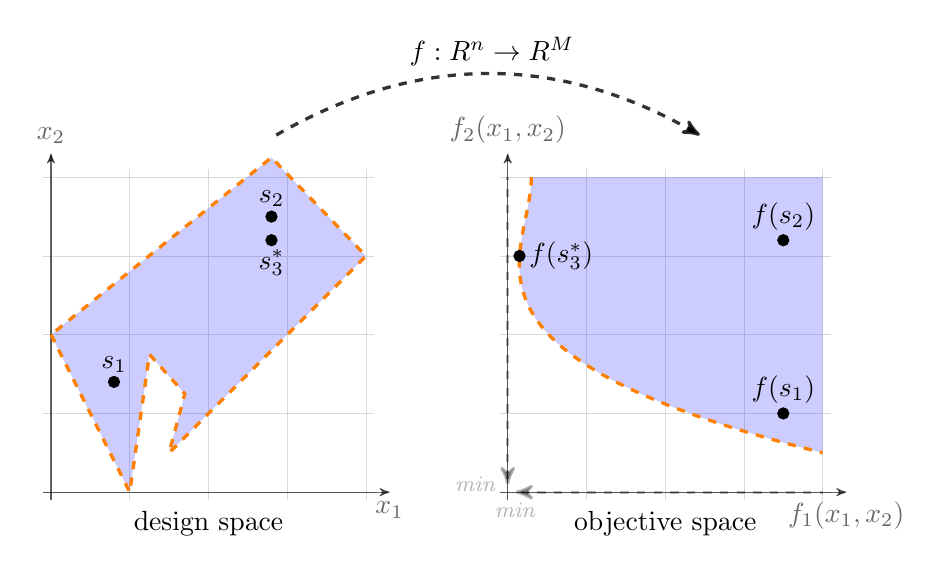
\begin{tikzpicture}
%      
        \tikzset{
          >=stealth',
          pil/.style={
            ->,
            thick,
            shorten <=2pt,
            shorten >=2pt,}
        }

        \begin{scope}[xshift=-5.8cm]
            \draw[very thin,color=gray, opacity=0.3]
              (-0.1,-0.1) grid (4.1,4.1);
            \draw[->, opacity=0.6] (-0.1,0) -- (4.3,0) node[below]
              {$x_1$};
            \draw[->, opacity=0.6] (0,-0.1) -- (0,4.3) node[above]
              {$x_2$};

            \begin{scope}
                \draw[dashed, very thick, fill=blue, fill opacity=0.2, draw=orange]
                  (0,2) -- (1,0) -- (1.25,1.75) --
                  (1.7,1.25) -- (1.5,0.5) -- (4,3) --
                  (2.8,4.25) -- (0,2);
            \end{scope}
            \draw (2.0, -0.4) node {design space};
      \end{scope}

      \begin{scope}
            \draw[very thin,color=gray, opacity=0.3]
              (-0.1,-0.1) grid (4.1,4.1);
            \draw[->, opacity=0.6] (-0.1,0) -- (4.3,0) node[below]
              {$f_1(x_1,x_2)$};
            \draw[->, opacity=0.6] (0,-0.1) -- (0,4.3) node[above]
              {$f_2(x_1,x_2)$};

            \draw[fill, color=blue, draw opacity=0, fill opacity=0.2]
              (0.3,4) .. controls (0.3,3)
              and (-1,1.75) .. (4.0,0.5)
              -- (4,4) -- (0.3,4);
            \draw[dashed, very thick, color=orange]
              (0.3,4) .. controls (0.3,3)
              and (-1,1.75) .. (4.0,0.5);

            \path[dashed, very thick, <-, opacity=0.3]
              (0.1,-0.0) edge (4.0,-0.0)
              node[below] {{\footnotesize\textit{min}}};
            \path[dashed, very thick, <-, opacity=0.3]
              (-0.0,0.1) edge (-0.0,4.0)
              node[left] {{\footnotesize\textit{min}}};
            \draw (2.0, -0.4) node {objective space};
      \end{scope}

      \path[pil, dashed, very thick, opacity=0.8]
      (-3.0,4.5) edge [bend left] (2.5,4.5);
      \path (-0.2,5.6) node {$f : \mathbb{R}^n \rightarrow \mathbb{R}^M$};

      \filldraw[] (-5,1.4) circle (2pt) node[above] {$s_1$};
      \filldraw[] (3.5,1)  circle (2pt) node[above] {$f(s_1)$};
      %\path[pil, dashed, very thick, red, opacity=0.7]
        %(-4.93,1.45) edge [bend left] (3.8,1.03);

      \filldraw[] (-3,3.5)  circle (2pt) node[above] {$s_2$};
      \filldraw[] (3.5,3.2) circle (2pt) node[above] {$f(s_2)$};
      %\path[pil, dashed, very thick, red, opacity=0.7]
        %(-2.93,3.55) edge [bend left] (3.73,3.23);

      \filldraw[] (-3,3.2)   circle (2pt) node[below] {$s_3^*$};
      \filldraw[] (0.15,3.0) circle (2pt) node[right] {$f(s_3^*)$};
      %\path[pil, dashed, very thick, blue, opacity=0.7]
        %(-2.93,3.25) edge [bend left] (0.08,3.03);


    \end{tikzpicture}
  \end{center}
  \caption{The (often non-linear) mapping $f : \mathbb{R}^n \rightarrow
    \mathbb{R}^M$ from design to objective space. The dashed lines represent
    the constraints in design space.
    %and the set of solutions (Pareto front) in objective space.
    }
  \label{fig:des_to_obj}
\end{figure}
\nomenclature{$\mathbb{R}$}{reel numbers}

A special subset of multi-objective optimization problems where all objectives
  and constraints are linear, called \textit{Multi-objective linear programs},
  exhibit formidable theoretical properties that facilitate convergence proofs.
In this thesis we strive to address arbitrary multi-objective optimization
  problems with non-linear constraints and objectives.
No general convergence proofs are readily available for these cases.


\section{Pareto Optimality}

In most multi-objective optimization problems we have to deal with conflicting
  objectives.
Two objectives are conflicting if they possess different minima.
If all the mimima of all objectives coincide the multi-objective optimization
  problem has only one solution.
To facilitate comparing solutions we define a partial ordering relation on
  candidate solutions based on the concept of dominance.
A solution is said to dominate another solution if it is no worse than the
  other solution in all objectives and if it is strictly better in at least
  one objective.
A more formal description of the dominance relation is given in
  Definition~\ref{def:dom}~\cite{deb:09}.

\begin{mydef} \label{def:dom}
A point $\mathbf{x}_1$ is dominating $\mathbf{x}_2$, if both properties
\begin{itemize}
  \item $f_m(\mathbf{x}_1) \geq f_m(\mathbf{x}_2) \text{,} \;\; \forall m \in
    \{ 1, \dots, M \}$
  \item $f_m(\mathbf{x}_1) > f_m(\mathbf{x}_2) \text{,} \;\; \exists m \in
    \{1, \dots, M\}$
\end{itemize}
hold. We denote this as $\mathbf{x}_1 \preceq \mathbf{x}_2$.
\end{mydef}
\nomenclature{$\preceq$}{dominance relation operator}

The properties of the dominance relation include transitivity
%
\begin{equation*}
  x_1 \preceq x_2 \wedge x_2 \preceq x_3 \Rightarrow x_1 \preceq x_3 \text{,}
\end{equation*}
%
  and asymmetricity, which is necessary for an unambiguous order relation
%
\begin{equation*}
  x_1 \preceq x_2 \Rightarrow x_2 \not\preceq x_1 \text{.}
\end{equation*}
%

Using the concept of dominance, the sought-after set of Pareto optimal
  solution points can be approximated iteratively as the set of non-dominated
  solutions.

The problem of deciding if a point truly belongs to the Pareto set is NP-hard.
As shown in Figure~\ref{fig:pareto-def} there exist ``weaker'' formulations of
  Pareto optimality.
Of special interest is the result shown in \cite{paya:01}, where the authors
  present a polynomial (in the input size of the problem and $1/\varepsilon$)
  algorithm for finding an approximation, with accuracy $\varepsilon$, of the
  Pareto set for database queries.

  \begin{figure}[tp]
  \begin{center}
%    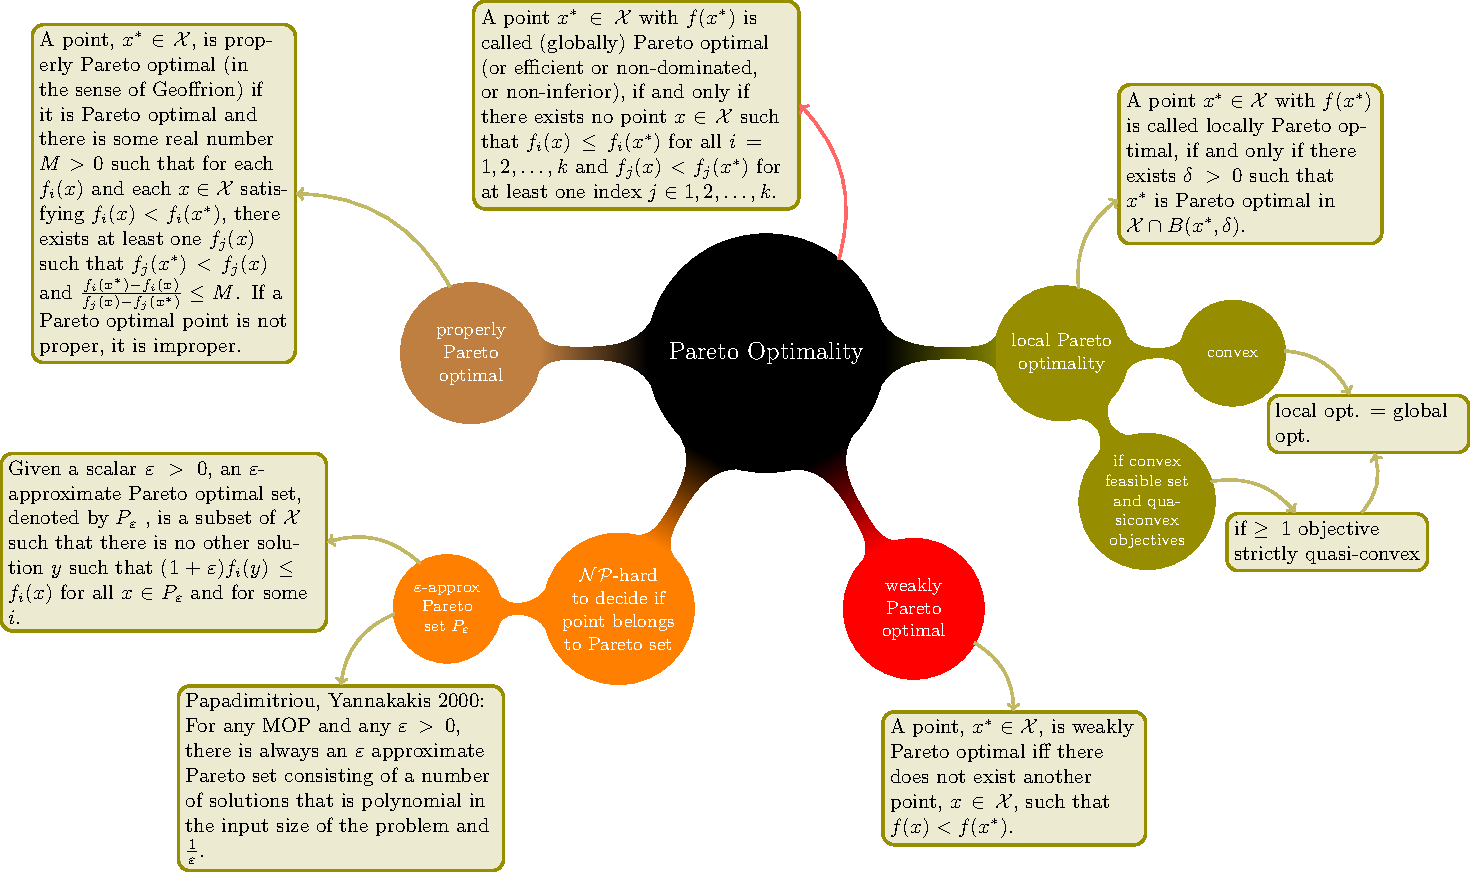
\includegraphics[angle=270,width=0.85\linewidth]{opt/pareto-defs.pdf}
  \end{center}
  \caption{Various definitions regarding Pareto optimality.}
  \label{fig:pareto-def}
\end{figure}





%----------- Footer control ------------------
\ifthenelse{\boolean{FullOPALManual}}
{
  %do nothing
}
% else (for individual document creation)
{
\appendix
\printbibliography
\end{document}
}
%---------------------------------------------